\section{Einleitung}
\label{sec:einleitung}

\begin{frame}
  \frametitle{Einleitung}

  \begin{itemize}
  \item Unterscheidung in 2 Kategorien
    \begin{itemize}
    \item Algorithmen zur Bestimmung der Position (Lokalisierung)
    \item Sinnvolle Positionierung der Sensoren
    \end{itemize}
  \end{itemize}
\end{frame}

\begin{frame}
  \frametitle{Einleitung - Lokalisierung}

  \begin{center}
    \textbf{Warum ist es wichtig, die eigene Position zu kennen?}\\~\\

    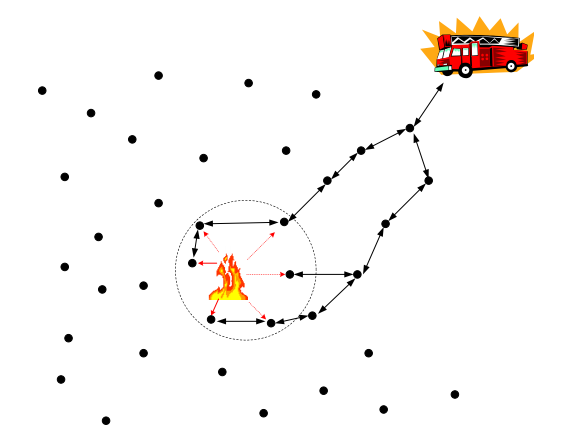
\includegraphics[scale=0.35]{img/lokalisierung_1}
  \end{center}
\end{frame}

\begin{frame}
  \frametitle{Einleitung - Positionierung}

  \begin{center}
    \textbf{Warum ist es wichtig, die Sensoren sinnvoll zu
      Positionieren?}\\~\\
  \end{center}

  % TODO Paper suchen und weitere Informationen hinzufügen,
  % verifizieren
  \begin{itemize}
  \item Wände können die Signale stark beeinträchtigen
  \item ...
  \end{itemize}
\end{frame}